\chapter{Machine Learning}\label{chap:MachineLearning}

In diesem Kapitel werden in \hyperref[sec:GrundlagenML]{Abschnitt 3.1} die für das weitere Verständnis der Arbeit nötigen Grundlagen zu \gls{ML} und in \hyperref[sec:DL]{Abschnitt 3.2} Grundlagen zu \gls{DL} vermittelt. Metriken zur Bewertung von \gls{ML}-Modellen werden in \hyperref[sec:metriken]{Abschnitt 3.3} eingeführt. Das Prinzip des Domain Shifts wird in \hyperref[sec:shift]{Abschnitt 3.4} erklärt.

\section{Grundlagen des Machine Learnings}\label{sec:GrundlagenML}

Unter \gls{ML} wird ein Prozess verstanden, bei welchem ein Computer aus gegebenen Daten ein statistisches Modell generiert, welches diese Daten abbildet und nach Beendigung der Lernphase gelernte Informationen auf andere Daten verallgemeinern kann. Angewendet wird so ein Modell bspw. für die Klassifikation von Daten in bestimmte Kategorien (bspw. ob ein \gls{EKG}-Abschnitt einen Sinusrhythmus darstellt oder nicht) oder im Falle eines Regressionsproblems für die Vorhersage kontinuierlicher Werte (bspw. die Wahrscheinlichkeit, mit welcher ein Patient \gls{VHF} entwickelt). \cite{nguyen_machine_2018} 

Klassifikation ist der Prozess, ungekennzeichneten Daten automatisch ein Label zuzuweisen. Ein Modell, das dieses Problem löst, heißt Klassifikator. Um ein solches Modell zu erzeugen, nutzt ein Klassifikations-Lernalgorithmus eine Datenmenge mit gelabelten (Supervised Learning) oder ungelabelten (Unsupervised Learning) Beispielen als Eingabe. Die Label bei einer Klassifikationsaufgabe sind Teil einer endlichen Menge von Klassen. Eine Klassifikationsaufgabe mit zwei Klassen nennt sich binäre Klassifikation, mit mehr Klassen wird von einer Multiklassen-Klassifikation gesprochen. \cite{burkov_machine_2019}

Beim Supervised Learning besteht die Datenmenge $\{(x_i, y_i)\}^{N}_{i=1}$ zur Modellerstellung aus gelabelten Beispielen. Ein gelabeltes Beispiel besteht aus einem Merkmalsvektor $x_i$ und einem Label $y_i$. Jede Dimension $j = 1,...,D$ des Merkmalsvektors ist ein einzelnes Merkmal $x^{(j)}$, dass das Beispiel in irgendeiner Weise beschreibt. Bei allen Beispielen in der Datenmenge enthalten die Merkmalsvektoren an derselben Position $j$ dieselbe Art Information (bspw. enthält $x^{(1)}$ das Geschlecht des jeweiligen Patienten). Das Label $y_i$ des Beispiels beschreibt die Ausgabe, die bei Verwendung des Merkmalsvektors als Eingabe in das vom Lernalgorithmus erzeugte Modell erwartet wird. Im Falle eines Klassifikationsalgorithmus ist das Label ein Element einer endlichen Menge $\{1,2,...,C\}$ von Klassen, wobei eine Klasse eine Kategorie beschreibt, der das Beispiel zugeordnet wird.
Die beiden oben genannten Probleme Klassifikation und Regression gehören zum Bereich des Supervised Learning. \cite{burkov_machine_2019} 

Beim Unsupervised Learning besteht die Datenmenge $\{(x_i)\}^{N}_{i=1}$ aus einer Menge ungelabelter Beispiele, wobei ein Beispiel wieder einen Merkmalsvektor $x_i$ enthält, jedoch kein Label \cite{burkov_machine_2019}. Das Ziel des Lernalgorithmus besteht in diesem Fall darin, den Merkmalsvektor als Eingabe zu nehmen und Informationen über die Datenmenge zu erzeugen. Beim sogenannten Clustering teilt das System bspw. die Datenmenge anhand ähnlicher Eigenschaften in verschiedene zusammenhängende Gruppen ein. \cite{nguyen_machine_2018}


\section{Deep Learning}\label{sec:DL}

\gls{DL} ist ein Teilgebiet des \gls{ML} und bezeichnet das Training von tiefen Neuronalen Netzen, also Neuronalen Netzen mit mehr als zwei Schichten zwischen Ein- und Ausgabeschicht. Algorithmen im klassischen \gls{ML} erzeugen sogenannte flache Modelle, indem Parameter direkt anhand der Merkmale der Trainingsbeispiele angepasst werden. Neuronale Netze hingegen erlernen Parameter anhand der Ausgaben der vorhergehenden Schichten. Ein Vorteil von \gls{DL} ist die selbstständige Merkmalsdetektion, sodass im Gegensatz zum klassischen \gls{ML} die Merkmale nicht aufwändig per Hand ausgewählt werden müssen. Jedoch sind \gls{DL}-Modelle im Gegensatz zu klassischen \gls{ML}-Modellen schwer interpretierbar, da die große Anzahl an Schichten es schwierig macht nachzuvollziehen, wie das Modell Entscheidungen trifft.  \cite{burkov_machine_2019}

Goettling et al. \cite{goettling_xecgarch_2024} und Jo et al. \cite{jo_explainable_2021} entwickeln Neuronale Netze mit dem Ziel, deren Entscheidungen nachvollziehbarer zu gestalten.

\subsection{Artificial Neural Network}

Ein \gls{ANN} besteht aus sogenannten künstlichen Neuronen, die in Schichten angeordnet sind. Ein Neuron 

\begin{equation}
\label{Neuron}
O = f(\sum_{j=1}^n x^{(j)} \cdot w^{(j)}+b)
\end{equation}

nimmt einen Merkmalsvektor $x_i = [x^{(1)},..., x^{(n)}]$, multipliziert ihn mit einem Gewichtsvektor $w_i = [w^{(1)},..., w^{(n)}]$, summiert die erhaltenen Werte auf, addiert den Bias $b$, leitet das Ergebnis durch eine Aktivierungsfunktion $f$ und gibt einen einzelnen Wert aus. 

Die Werte der Gewichte (und des Bias) sind die Parameter, die beim Trainieren des Lernalgorithmus erlernt werden. Die Aktivierungsfunktion wird auf die gewichtete Summe aller Eingaben angewandt und fügt dem Neuron die Nichtlinearität hinzu. Sie wird vor dem Training festgelegt, häufig ist es eine der folgenden Funktionen:


\begin{align}
\label{sigmoid}
\text{Sigmoid: } &\quad f(z) = \frac{1}{1+e^{-z}} \\[1em]
\label{tanh}
\text{Tangens hyperbolicus: } &\quad f(z) = \frac{e^z - e^{-z}}{e^z + e^{-z}} \\[1em]
\label{relu}
\text{Rectified Linear Unit: } &\quad f(z) = 
\begin{cases} 
0, & \text{wenn } z < 0 \\ 
z & \text{sonst}
\end{cases}
\\[1em]
\label{softmax}
\text{Softmax: } &\quad f(z) = [f^{(1)},...,f^{(C)}]\text{, wobei } f^{(j)} = \frac{e^{z^{(j)}}}{\sum_{k=1}^C e^{z^{(k)}}}
\end{align}

Die Ausgabe der Softmax-Funktion beschreibt die Wahrscheinlichkeitsverteilung der verschiedenen Klassen C. Die Summe aller Ausgaben $f^{(1)},...,f^{(C)}$ ergibt 1.  Werden mehrere Neuronen zusammengeschaltet erhält man ein \gls{ANN}. In einem \gls{ANN} gibt es eine Eingabeschicht, eine Ausgabeschicht, sowie beliebig viele Schichten zwischen diesen, welche als Hidden Layer bezeichnet werden. Hat ein \gls{ANN} viele Hidden Layer, wird es auch als \gls{DNN} bezeichnet. \cite{burkov_machine_2019}

Es gibt verschiedene Architekturen von \glspl{ANN}. Die simpelste Architektur eines \glspl{ANN} ist das \gls{FFNN} (auch Multilayer Perceptron) \cite{murphy_probabilistic_2022}. In einem \gls{FFNN} existieren keine Schleifen und es gibt einen direkten Weg von Eingabe- zu Ausgabeschicht (siehe \hyperref[fig:ANN]{Abb.~3.1}). Als fully connected bezeichnet man die Schichten, wenn alle Neuronen der Schicht voneinander unabhängig sind, jedes Neuron alle Ausgaben der vorherigen Schicht als Eingaben erhält und seine Ausgaben an alle Neuronen der nachfolgenden Schicht weitergibt. \cite{nielsen_neural_2015}

%\begin{figure}[!ht]%
%\centering
%	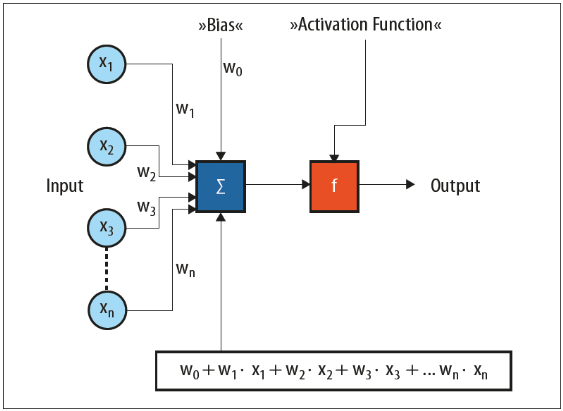
\includegraphics[width=0.80\textwidth]{./Bilder/artificial_neuron.png}
%	\caption[Künstliches Neuron]{Ein künstliches Neuron mit den Eingabewerten %$x_1$ bis $x_n$ und den zugehörigen Gewichten $w_1$ bis $w_n$, sowie dem mit $w_0$ gewichteten Bias, welche aufsummiert und durch die Aktivierungsfunktion $f$ geleitet werden. Ausgegeben wird ein einzelner Wert. Entnommen aus \cite{nguyen_machine_2018}.}
%\label{fig:Neuron}
%\end{figure}

\begin{figure}[!ht]%
\centering
	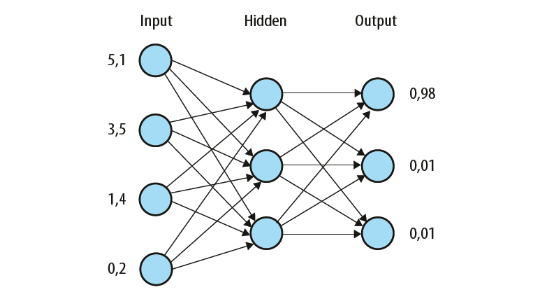
\includegraphics[width=0.80\textwidth]{./Bilder/ANN.png}
	\caption[Feed Forward Neural Network]{Ein Feed Forward Neural Network mit einem fully connected Hidden Layer und beispielhaften Eingangs- und Ausgangswerten. Entnommen aus \cite{nguyen_machine_2018}.}
\label{fig:ANN}
\end{figure}

\subsection{Convolutional Neural Network}

Ein \gls{CNN} ist ein \gls{FFNN}, welches häufig zur Bildverarbeitung eingesetzt wird und gut für Mustererkennung geeignet ist. Es besitzt sogenannte Convolutional Layer, in denen Filter vorhanden sind. Diese Filter sind kleine Matrizen, die jeweils ein anderes Muster erkennen. Dies tun sie, in dem sie stückweise über die Bildmatrix geschoben werden und mit dem Bildausschnitt (Patch) gefaltet werden, den sie überlagern. Je ähnlicher sich Filtermatrix und Patch sind, desto größer ist der Wert, der bei der Convolution erhalten wird. Ein Convolutional Layer in einem \gls{CNN} besteht aus mehreren Filtern, deren Ergebnis jeweils ein Bias-Parameter hinzugefügt wird, bevor die Aktivierungsfunktion angewendet wird. Die Filtermatrix und die Bias-Parameter sind trainierbare Werte in einem \gls{CNN}. Convolutions besitzen eine Schrittweite, die angibt wie weit die Filtermatrix bei jedem Schritt geschoben wird, und ein Padding, welches dem Rand des Bildes hinzugefügt werden kann, damit dieser besser erkennbar ist. Als Aktivierungsfunktion wird üblicherweise die Rectified Linear Unit (ReLu)-Funktion genutzt. Je tiefer der Convolutional Layer ist, desto komplexer werden die Muster, die ein Filter erkennen kann. CNNs besitzen sogenannte Pooling Layer. Ein Pooling Layer folgt üblicherweise auf ein Convolutional Layer. Beim Max-Pooling wird ähnlich wie bei einer Convolution ein Fenster mit einer bestimmten Schrittweite über eine Eingabematrix geschoben, aber anstatt eine Convolution durchzuführen wird der größte Wert im Fenster ausgewählt und ausgegeben. \cite{burkov_machine_2019}

 
Je tiefer ein \gls{DNN} ist, desto schwieriger ist es zu trainieren, da das Degradationsproblem auftritt. Dies bedeutet, dass mit einer zunehmenden Anzahl an Schichten die Genauigkeit eines Modells ab einem bestimmten Punkt gesättigt ist und von da an beginnt zu sinken. Ein Modell mit weniger Schichten hat also eine bessere Leistung als ein Modell mit mehr Schichten, obwohl Letzteres in der Lage sein sollte, komplexere Muster zu erkennen. Ein Grund hierfür kann das \textit{Vanishing Gradient Problem} sein. \textit{Backpropagation} ist ein Algorithmus zur Aktualisierung der Parameterwerte von \gls{ANN}s, mit welchem effizient der Gradient der \gls{ANN}s berechnet werden kann \cite{burkov_machine_2019}. Beim Vanishing Gradient Problem werden während der Backpropagation die Gradienten sehr klein und die Gewichte der vorderen Schichten ändern sich deshalb nicht mehr. 
\glspl{ResNet} lösen das Degradationsproblem, indem sie sogenannte Residualverbindungen (auch Skip oder Shortcut Connections genannt) nutzen, um Schichten zu überspringen. Ein \gls{ResNet} besteht aus mehreren Residual Blocks, welche wiederum aus zwei oder mehr Convolutional Layern bestehen. Die Residual Blocks sind durch Shortcut Connections so verbunden, dass die Eingabe des einen Residual Blocks direkt mit seiner Ausgabe addiert wird und dies als Eingabe für den nächsten Block gilt. Die Shortcut Connections ermöglichen eine effektivere Gradientenweiterleitung während der Backpropagation und ermöglichen das Training tieferer Modelle. \cite{he_deep_2015}

\subsection{Training von Lernalgorithmen}

Das Trainieren eines Lernalgorithmus ist im Grunde das Lösen einer Optimierungsaufgabe. 
Jeder Lernalgorithmus besitzt eine Verlustfunktion (engl. Loss Function), die auch als Fehler bezeichnet wird. Sie ist das Maß dafür, wie stark sich die Ausgabe des Lernalgorithmus von dem tatsächlichen Label unterscheidet. Parameter sind Variablen im erzeugten Modell, deren Werte vom Lernalgorithmus während des Trainings erlernt werden. Sie werden auch als Gewicht und Bias bezeichnet. Gewichte stellen die Stärke der Verbindung zwischen den Neuronen dar und beeinflussen somit, wie stark oder schwach ein Eingangssignal das Neuron aktiviert und wie stark es zur Ausgabe beiträgt. Das Bias ist ebenfalls ein Gewicht, jedoch ist es eine Konstante und ermöglicht es dem Neuron, auch dann aktiviert zu werden, wenn alle Eingaben null sind. 
Die Optimierungsaufgabe besteht darin, die Parameter des Modells iterativ so anzupassen, dass der Wert der Loss Function minimiert wird, sich also die Ausgabe des Lernalgorithmus so gut wie möglich mit dem tatsächlichen Label deckt. \cite{burkov_machine_2019}

Eines der am häufigsten angewandten Verfahren, welches zur Optimierung genutzt wird, ist der Gradientenabstieg (engl. Gradient Descent). Mit ihm kann iterativ das Minimum (oder Maximum) der Loss Function und damit die optimalen Parameterwerte gesucht werden. Eine Iteration wird als Epoche bezeichnet. Der Gradient Descent beginnt mit zufällig ausgewählten Werten für die Parameter. Anschließend wird mit Hilfe der Ableitung die Steigung der Kurve der Loss Function am Punkt der aktuellen Parameterwerte berechnet. Ist die Steigung positiv, werden die Parameterwerte in der nächsten Epoche reduziert, der Punkt wird also im Graphen nach links bewegt. Ist die Steigung negativ, werden die Parameterwerte in der nächsten Epoche erhöht, der Punkt wird also im Graphen nach rechts bewegt. Die Größe dieser Bewegung wird durch die Lernrate (engl. Learning Rate) definiert. Anschließend wird der Vorgang mit den neuen Parameterwerten so oft iteriert, bis ein Abbruchkriterium erfüllt ist. Sobald die Steigung null ist, wurde ein Minimum und somit optimale Parameterwerte gefunden. Allerdings kann es sich dabei um ein lokales Minimum handeln, welches nicht unbedingt bedeutet, dass die absolut optimalen Parameterwerte gefunden wurden. Lokale Minima lassen sich bspw. durch eine dynamische Anpassung der Learning Rate vermeiden. \cite{nguyen_machine_2018}

Der stochastische Gradientenabstieg (engl. Stochastic Gradient Descent) ist eine Version des Gradient Descent, der den Gradienten näherungsweise mit Teilmengen der Trainingsdatenmenge berechnet und so die Berechnung beschleunigt. Beim Training von \gls{ANN}s werden häufig die Varianten \textit{RMSprop} oder \textit{Adam} des Stochastic Gradient Descent genutzt. \cite{burkov_machine_2019}

\subsection{Optimierung der Hyperparameter} 

Hyperparameter werden nicht durch den Lernalgorithmus selbst optimiert und müssen mit einem anderen Verfahren optimiert werden. Wenn die verfügbare Datenmenge groß genug, in der Validierungsmenge jede Klasse in einer ausreichenden Anzahl vertreten und die Anzahl der Hyperparameter sowie deren Wertebereich nicht zu groß ist, kann Rastersuche (engl. Grid Search) genutzt werden. Hierbei werden für jeden Hyperparameter Werte bspw. anhand einer logarithmischen Skala festgelegt. Anschließend werden verschiedene Kombinationen der Hyperparameterwerte zusammengestellt und es wird für jede dieser Kombinationen mit der Trainingsmenge ein Modell erstellt. Anschließend wird die Leistung der Modelle beurteilt. Wenn die optimalen Hyperparameterwerte gefunden wurden, können zusätzlich Werte in der Nähe ausprobiert werden, da sich unter Umständen noch bessere Hyperparameterwerte ergeben können. \cite{burkov_machine_2019}

Bei der Zufallssuche (engl. Random Search) werden im Gegensatz zur Grid Search keine diskreten Wertemengen für die Hyperparameter zusammengestellt, sondern es wird für jeden Hyperparameter eine statistische Verteilung vorgegeben, aus welcher Werte entnommen werden und festgelegt, wie viele Wertekombinationen ausprobiert werden sollen \cite{burkov_machine_2019}. 


\section{Bewertung von Klassifikatoren}\label{sec:metriken}

Die Datenmenge kann in drei Teilmengen aufgeteilt werden: Trainingsmenge, Validierungsmenge und Testmenge. Um den Klassifikator zu validieren, gibt es zwei geläufige Ansätze: Die Holdout-Validierung und die Kreuzvalidierung (engl. Cross Validation). Für die Validierung werden Daten benötigt, die nicht zum Training beigetragen haben. Bei der Holdout-Validierung ist die Trainingsmenge im Idealfall die größte dieser Teilmengen und wird für das Training genutzt. Validierungs- und Testmenge sind sogenannte Holdout-Datenmengen. Sie sind im Idealfall wesentlich kleiner und tragen nicht zum Training bei. Zu beachten ist, dass bei einer insgesamt kleinen Validierungs- und Testmenge die zugrundeliegende Verteilung der Daten unter Umständen nicht vollständig abgebildet wird, sodass die Ergebnisse aus Validierung und Test weniger aussagekräftig sind. Die Validierungsmenge wird verwendet, um den besten Lernalgorithmus auszuwählen und die besten Werte für die Hyperparameter zu ermitteln. Bei der Cross Validation wird die Datenmenge nur in Trainings- und Testmenge aufgeteilt. Die Trainingsmenge wird wiederum in $n$ Mengen aufgeteilt. Anschließend werden $n-1$ Modelle trainiert, wobei jeweils $n-1$ Mengen zum Training und die $n-te$ Menge zur Validierung genutzt wird. In beiden Fällen wird die Testmenge  genutzt, um das finale Modell zu beurteilen, bevor es produktiv eingesetzt wird. \cite{burkov_machine_2019}

Bei dem Erstellen eines Modells können verschiedene Probleme auftreten. Wenn das Modell nicht genug an die Daten angepasst ist, kommt es zur sogenannten Unteranpassung (engl. Underfitting), das Modell hat ein hohes Bias. Das Modell macht also sowohl bei der Vorhersage von Labeln der Trainingsdaten als auch bei denen der Testdaten viele Fehler. Ursache hierfür kann u.A. sein, dass ein zu einfaches Modell gewählt wurde oder die erstellten Merkmale nicht aussagekräftig genug sind. Sagt das Modell die Label der Trainingsdaten sehr gut vorher, aber die der Testdaten nur sehr schlecht, besteht eine Überanpassung (engl. Overfitting), das Modell hat eine hohe Varianz. Dies kann durch ein zu komplex gewähltes Modell auftreten oder dadurch, dass zu viele Merkmale bei nur wenigen Trainingsbeispielen vorliegen. Um die Generalisierbarkeit des Modells zu gewährleisten, sollten die Trainingsdaten eine ausreichende Diversität aufweisen. Dadurch wird vermieden, dass das Modell sich nur an spezifische Eigenheiten der Trainingsdaten anpasst, was ebenfalls zu Overfitting führen kann. Zusätzlich müssen die Testdaten möglichst unabhängig von den Trainingsdaten sein, um eine realistische Einschätzung der Modellleistung auf bisher unbekannten Daten zu ermöglichen.  \cite{burkov_machine_2019}

\subsection{Metriken zur Bewertung der Klassifikationsgüte}
Um festzustellen, ob das Modell Klassen von Daten gut vorhersagen kann, die dem Lernalgorithmus unbekannt sind, gibt es bestimmte Metriken, die in diesem Abschnitt vorgestellt werden.

\subsubsection*{Confusion Matrix}
In einer binären Klassifikationsaufgabe mit den Labeln \textit{positiv} und \textit{negativ} kann man im allgemeinen vier Fälle unterscheiden:
\begin{itemize}
\item \gls{TP}: Anzahl der korrekt als positiv vorhergesagten Label
\item \gls{FP}: Anzahl der fälschlicherweise als positiv vorhergesagten Label
\item \gls{FN}: Anzahl der fälschlicherweise als negativ vorhergesagten Label
\item \gls{TN}: Anzahl der korrekt als negativ vorhergesagten Label
\end{itemize}

Die Matrix in der sie eingetragen werden nennt sich Confusion Matrix (Wahrheitsmatrix).
Ziel ist, die Werte für \gls{TP} und \gls{TN} zu maximieren. Diese Fälle können auch auf Multiklassen-Klassifikationen erweitert werden. \cite{nguyen_machine_2018}

\subsubsection*{Accuracy}

Die Accuracy (Korrektklassifikationsrate) gibt das Verhältnis der Anzahl richtiger Vorhersagen der Labels zur Menge aller untersuchten Beispiele als 
\begin{equation}
\label{eq:accuracy}
Accuracy = \frac{TP+TN}{TP+FP+TN+FN}
\end{equation} \cite{nguyen_machine_2018} an. 


\subsubsection*{Precision-Recall}

Die Precision (Genauigkeit) wird angegeben als \begin{equation}
\label{eq:precision}
Precision = \frac{TP}{TP+FP}
\end{equation} und stellt das Verhältnis der richtigen positiven Vorhersagen zu den positiven Vorhersagen insgesamt dar.  



Recall (auch Sensitivity, Trefferquote oder True-positive-rate) ist das Verhältnis der richtigen positiven Vorhersagen zu den insgesamt in der Datenmenge vorhandenen positiven Beispielen:
\begin{equation}
\label{eq:recall}
Recall = \frac{TP}{TP+FN}
\end{equation}.

Es kann eine Precision-Recall-Kurve generiert werden und anhand der Fläche unter der Kurve (\gls{AUC}) beurteilt werden, wie gut Precision und Recall gleichzeitig sind. Um gute Werte sowohl für Precision als auch für Recall auszuwählen, wird der F1-Score genutzt. Der F1-Score wird entsprechend \begin{equation}
\label{eq:F1}
F1 = \frac{2 \cdot Precision \cdot Recall}{Precision + Recall}
\end{equation} berechnet und ist das harmonische Mittel zwischen Precision und Recall. \cite{nguyen_machine_2018}


\subsubsection*{Specificity}

Die Specificity oder auch True-negative-rate gibt das Verhältnis der richtigen negativen Vorhersagen zu den insgesamt in der Datenmenge vorhandenen negativen Beispielen als
\begin{equation}
\label{eq:specificity}
Specificity = \frac{TN}{TN+FP}
\end{equation}
an.

\subsubsection*{Receiver-Operating-Characteristic-Kurve}

In der \gls{ROC} Kurve wird die Fallout-Rate (False-positive-rate) $fp/(fp+tn)$ gegen den Recall eingetragen. Die Fläche unter der Kurve (\gls{AUC}) ist ein Maß für die Leistung des Modells. \cite{burkov_machine_2019}

\section{Domain Shift}\label{sec:shift}

In der Praxis trifft ein Modell oft auf veränderte Bedingungen: Die Daten, auf denen es trainiert wurde, unterscheiden sich häufig von denen, die es später in der Anwendung sieht. Dieses Phänomen wird Domain Shift genannt \cite{dissanayake_domain_2021}. Ein Domain Shift tritt auf, wenn die Datenverteilung, auf denen ein Modell trainiert wurde (Quelldomäne), unterschiedlich zur Verteilung der Daten, die das Modell in der Praxis sieht (Zieldomäne), ist. Dies führt zu einem Leistungsabfall des Modells. Der Begriff Datenverteilung bezieht sich hierbei auf die statistischen Eigenschaften und Merkmale der Daten insgesamt, nicht nur auf die Häufigkeit der Klassen. \cite{wang_generalizing_2023}

Mathematisch lässt sich eine Domäne $\mathcal{S}$ beschreiben als eine Kombination von Merkmalen $x$ aus einem Eingaberaum $\mathcal{X}$ und Labeln $y$ aus einem Ausgaberaum $\mathcal{Y}$, mit einer zugehörigen Datenverteilung $P_{XY}$. Dies wird als 
\begin{equation}
\mathcal{S} = {(x_i,y_i)^n_{i=1}} \sim P_{XY}
\end{equation}
notiert. $X$ und $Y$ beschreiben die zugehörigen Zufallsvariablen. Die bekanntesten Lösungsansätze für das Domain Shift-Problem sind Transfer Learning, \gls{DAp} und \gls{DG}. \cite{wang_generalizing_2023}

\subsection{Domain Adaptation und Transfer Learning}

Beim Transfer Learning können die Domänen sich in Merkmalsraum, Labelraum und/oder Datenverteilung unterscheiden. \gls{DAp} beschreibt den konkreteren Fall, bei welchem sich die Domänen nur in ihrer Datenverteilung unterscheiden. Da dieser Fall beim Transfer Learning mit inbegriffen ist, kann \gls{DAp} mittels Transfer Learning erreicht werden. \cite{kouw_introduction_2019}

Bei der \gls{DAp} wird ein Modell bspw. mittels Pretraining-Finetuning zuerst auf eine eine Quelldomäne $\mathcal{S}^{src}$ trainiert und anschließend auf eine Zieldomäne $\mathcal{S}^{tar}$ angepasst. Sowohl beim Transfer Learning als auch bei der \gls{DAp} besteht während des Trainings Zugriff auf Daten aus der Zieldomäne $\mathcal{S}^{tar}$. \cite{wang_generalizing_2023} 

\subsection{Domain Generalization}
 
Das Ziel der \gls{DG} ist, ein Modell auf eine oder mehrere unterschiedliche, aber verwandte Domänen $\mathcal{S}^1,...,\mathcal{S}^n$ zu trainieren, sodass es gut auf unbekannte Domänen $\mathcal{S}^{n+1}, \mathcal{S}^{n+2},...$ verallgemeinern kann. Im Gegensatz zur \gls{DAp} besteht während des Trainings kein Zugriff auf Daten aus den Zieldomänen, sodass \gls{DG} zwar ein komplexerer, aber auch ein Ansatz näher an der tatsächlichen Praxis ist. \cite{wang_generalizing_2023}

Methoden für \gls{DG} lassen sich aufteilen in Data Manipulation-basierte Methoden, Representation Learning-basierte Methoden und allgemeine Lernstrategien, die zur \gls{DG} beitragen. Diese Methoden lassen sich kombinieren, um eine noch bessere \gls{DG} zu erreichen. \cite{wang_generalizing_2023}

\subsubsection*{Data Manipulation-basierte Methoden}

Die Kategorie der Data Manipulation-basierten Methoden konzentriert sich auf die Veränderung der Eingabedaten, um die Diversität und Quantität der existierenden Trainingsdaten zu erhöhen, wodurch ein Overfitting reduziert und damit die Fähigkeit des Modells zu Generalisieren erhöht wird. Bei der Data Augmentation werden vorhandene Daten mit Rauschen erweitert, rotiert, zugeschnitten, skaliert oder anderweitig transformiert. Bei der Data Generation werden Daten bspw. mittels eines Generative Adversarial Networks künstlich erzeugt. \cite{wang_generalizing_2023} 

\subsubsection*{Representation Learning-basierte Methoden}

Beim Representation Learning geht es darum, dass Modelle Merkmale erlernen, die die Eingabedaten möglichst gut repräsentieren. Es gibt dazu zwei Lernstrategien, die gut zur \gls{DG} geeignet sind, nämlich Domain Invariant Representation Learning und Feature Disentanglement. 

Beim Feature Disentanglement werden Merkmale in domäneninvariante und domänenspezifische Merkmale getrennt. 
Beim Domain Invariant Representation Learning ist das Ziel, domänenunabhängige Merkmale zu extrahieren. Dies kann bspw. durch Domain Adversarial Learning (siehe \hyperref[sec:DAL]{Abschnitt. 3.4.3}) oder Explicit Feature Alignment erreicht werden. Bei Letzterem wird darauf abgezielt, Merkmalsverteilungen zwischen verschiedenen Domänen explizit anzugleichen. \cite{wang_generalizing_2023} 




\subsubsection*{Allgemeine Lernstrategien zur \gls{DG}}

Es gibt allgemeine \gls{ML} Paradigmen, die sich gut für \gls{DG} eignen. Eine gut geeignete Lernstrategie ist das Ensemble Learning. Hierbei werden mehrere Klassifikatoren trainiert und das Ergebnis bspw. anhand einer Mehrheitsentscheidung aller Modelle bestimmt. Ein Ensemble hat den Vorteil, dass durch die Diversität der Modelle die Gesamtleistung erhöht wird. \cite{wang_generalizing_2023} 

%TODO
 %- Meta Learning
 %- Gradient Operation
 %- Self Supervised Learning
 %- Distributionally Robust Optimization
 
 
Der in dieser Arbeit vorgestellte Ansatz vereint die zwei \gls{DG} Methoden Domain Adversarial Learning und Ensemble Learning.

\subsection{Domain Adversarial Learning}\label{sec:DAL}

Ganin et al. \cite{ganin_domain-adversarial_2016} haben den Ansatz des Domain Adversarial Learnings ursprünglich als Methode zur \gls{DAp} entwickelt. Sie stützen sich hierbei auf die Hypothese, dass die Vorhersagen eines Modells auf Merkmalen getroffen werden müssen, die unabhängig von Quell- und Zieldomäne sind, um den Domain Shift zu überwinden.
Der Ansatz von Ganin et al. nutzt gelabelte Daten aus der Quelldomäne und nicht-gelabelte Daten aus der Zieldomäne und zielt darauf ab, dass Merkmale erlernt werden, die differenzierend für die Hauptklassifikationsaufgabe fungieren, jedoch unempfindlich gegenüber dem Domain Shift sind. 

Ganin et al. führen aus, dass ihr Ansatz mit beinahe jedem \gls{FFNN} funktioniert und das Training mit den Standardmethoden Backpropagation und Gradientenabstieg durchgeführt werden kann.
Die Architektur (\hyperref[fig:DANN_prinzip]{siehe Abb.~3.2}) eines \glspl{DANN} besteht aus einem \textit{Feature Extractor} und einem \textit{Label Predictor}, die zusammen ein Standard-\gls{FFNN} bilden, sowie einem \textit{Domain Classifier}, der mit dem Feature Extractor durch ein \gls{GRL} verbunden ist. Der \gls{GRL} multipliziert den Gradienten während der Backpropagation mit einem konstanten negativen Wert. Die Gradientenumkehr führt dazu, dass das Modell lernt, die Domänen möglichst schlecht zu unterscheiden. \cite{ganin_domain-adversarial_2016}

\begin{figure}[!ht]%
\centering
	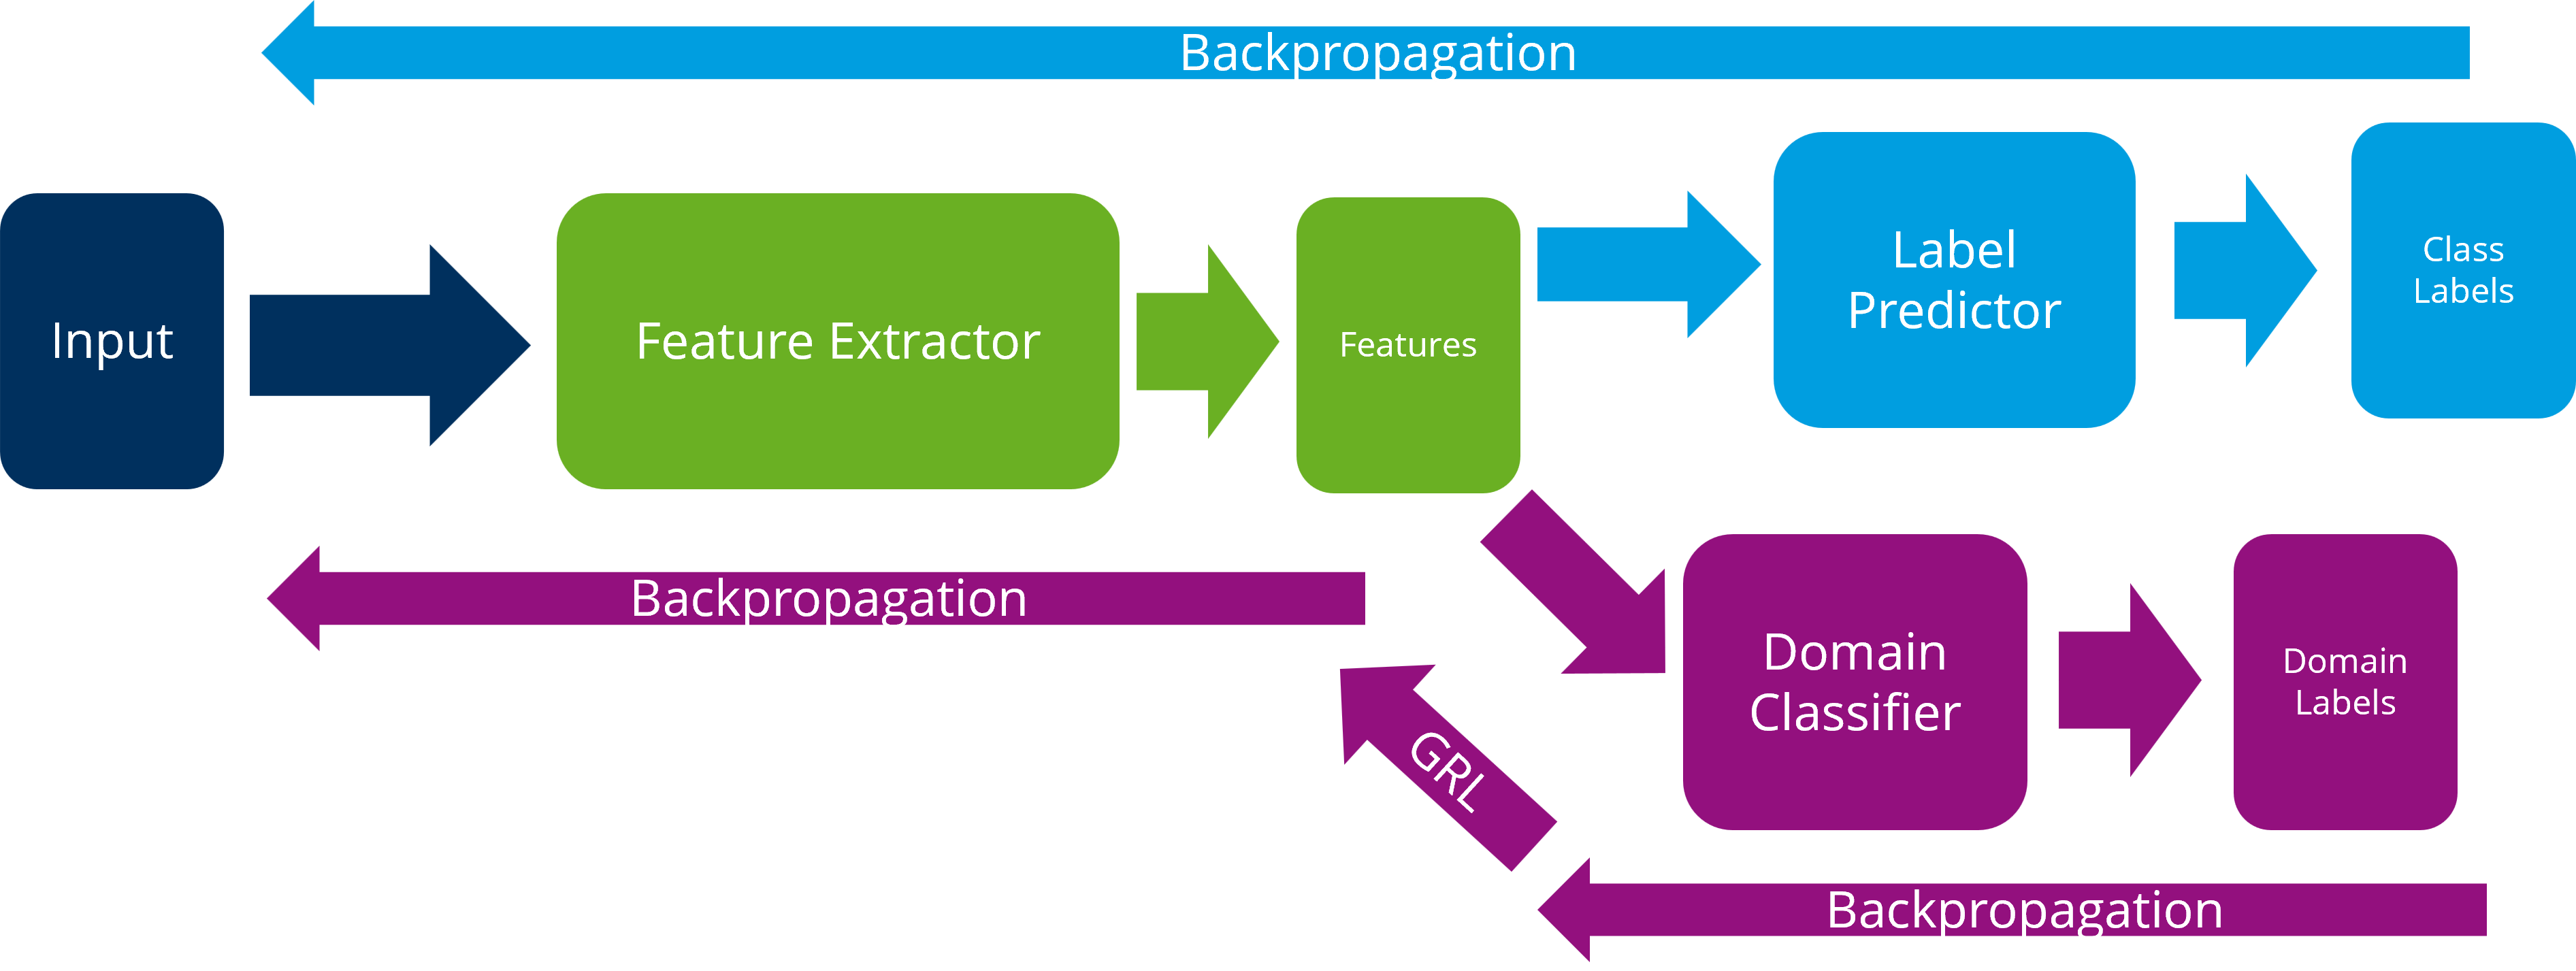
\includegraphics[width=1.0\textwidth]{./Bilder/DANN_aufbau.png}
	\caption[Domain Adversarial Nerual Network Prinzip]{Ein Domain Adversarial Neural Network nach \cite{ganin_domain-adversarial_2016}. Es besteht aus einem Feature Extractor, einem Label Predictor und einem Domain Classifier. Der Gradient des Domain Classifiers wird während der Backpropagation durch den Gradient Reversal Layer (GRL) invertiert. }
\label{fig:DANN_prinzip}
\end{figure}

